\section{Thuật toán chính xác}

\subsection{Nhánh và cận}

Một trong những thuật toán chính xác được nghiên cứu sớm nhất là \textit{nhánh và cận}, lần đầu xuất hiện trong bài báo \textit{"An Algorithm for the Vehicle Dispatching Problem"} của N. Christofides và S. Eilon năm 1969 \cite{christofides1969algorithm}. Với $m$ là tham số đầu vào, đầu tiên đồ thị được mở rộng với việc thêm vào $m-1$ kho ảo và đặt chi phí của chúng bằng một số vô cùng lớn. Sau đó giải bài toán m-TSP trên đồ thị này bằng thuật toán TSP được trình bày bởi Little et al. (1963) \cite{little1963algorithm}

Hiệu năng của các thuật toán nhánh-cận đầu tiên được cải thiện đáng kể hai phương pháp cận dưới là k-degree centre trees (k-DCT) và q-routes (Christofides et al. (1981) \cite{christofides1981exact}).

\subsection{Quy hoạch động}

Eilon, Watson-Gandy và Christofides (1971) \cite{christofides1969algorithm} đưa ra lời giải cho bài toán VRP bằng phương pháp quy hoạch động. Gọi $c(S)$ là chi phí tối ưu của một tuyến ứng với tập nút $S \subseteq V \setminus \{0\}$. Mục tiêu là cực tiểu hóa $\sum_{r=1}^{m} c(S_r)$ trên tất cả các quy hoạch khả dĩ $\{S_1,...,S_m\}$ của $V \setminus \{0\}$. Gọi $f_k(U)$ là chi phí nhỏ nhất có thể đạt được khi sử dụng $k$ xe cho một tập con $U$ của $V \setminus \{0\}$. Ta có
\begin{equation}
	\label{eq:dp}
	f_k(U) =
	\begin{cases}
		c(U) \quad \text{nếu } k = 1,                                                                                      \\
		\min_{U^* \subseteq U \subseteq V \setminus \{0\}} \{f_{k-1} (U \setminus U^*) + c(U^*)\} \quad \text{nếu } k > 1. \\
	\end{cases}
\end{equation}
Chi phí tối ưu là $f_m(V \setminus \{0\})$ và các tuyến là các phân hoạch của $V \setminus \{0\}$ theo phương trình (\ref{eq:dp}).

\subsection{Công thức  dòng xe và thuật toán}
Công thức 2-chỉ số cho bài toán VRP được nghiên cứu đầu tiên bởi Laporte, Nobert (1983) \cite{laporte1983branch} và Laporte, Nobert, Desrochers (1985) \cite{laporte1985optimal} và mở rộng công thức TSP cổ điển của Dantzig, Fulkerson, Johnson (1954) \cite{dantzig1954solution}. Gọi $x_{ij}$ là biến 0-1-2 bằng số lần một xe đi qua cung $(i,j)$. Bài toán được mô hình hóa như sau
\begin{equation}
	\min \sum_{(i,j) \in E} c_{ij} x_{ij}
\end{equation}
s.t.
\begin{flalign}
	\label{ct2:1} & \sum_{j=1}^n x_{0j}=2m, & \quad \\
	\label{ct2:2} & \sum_{i<k} x_{ik} + \sum_{j>k} x_{kj} = 2, & \quad k \in V \setminus \{0\}, \\
	\label{ct2:3} & \sum_{i,j \in S} x_{ij} \leq |S| - \nu(S), & \quad S \subseteq V \setminus \{0\}, \\
	\label{ct3:3} & x_{0j} \in \{0,1,2\}, & \quad j \in V \setminus \{0\}, \\
	\label{ct2:4} & x_{ij} \in \{0,1\}, & \quad i,j \in V \setminus \{0\},
\end{flalign}
trong đó $\nu(S)$ là cận dưới của số lượng xe cần thiết để phục vụ tập $S$. Công thức dòng xe và các biến thể đã được trình bày kĩ từ chương \ref{chap:model}.

\subsection{Công thức dòng hàng và thuật toán}
Trong công thức dòng hàng, biến $y_{ij}$ (hoặc $y_{ijk}$) định nghĩa tải (lượng hàng) của xe mang theo trên cung $(i,j)$. Ví dụ được trình bày bởi Gavish, Graves (1979) \cite{gavish1978travelling}, tuy nhiên các tác giả không đưa ra kết quả tính toán. Các ví dụ gần đây hơn được nghiên cứu bởi Baldacci, Hadjiconstantinou, Mingozzi (2004) \cite{baldacci2004exact} dựa trên mô hình TSP của Finke, Claus, Gunn
(1984) \cite{finke1984two}. Công thức cho một đồ thị mở rộng $\bar{G} = (\bar{V}, \bar{E})$, với $\bar{V} = V \cup \{ (i, n+1): i \in V \}$. Một tuyến được định nghĩa là một đường đi có hướng từ $0$ đến $n+1$. Biến nhị phân $x_{ij}$ bằng $1$ khi và chỉ khi cạnh $(i,j)$ được chọn vào tuyến. Biến $y_{ij}$ định nghĩa tải của xe trên cung $(i,j)$ và $y_{ji} = Q - y_{ij}$ biểu diễn xe rỗng trên cung $(j,i)$ mỗi khi $x_{ij} = 1$. Công thức dòng hàng được mô hình hóa như sau

\begin{equation}
	\min \sum_{(i,j) \in E} c_{ij} x_{ij}
\end{equation}
s.t.
\begin{flalign}
	\label{ct3:1} & \sum_{j \in \bar{V}} (y_{ji} - y_{ij}) = 2q_i, & \quad i \in V \setminus \{0\}, \\
	\label{ct3:2} & \sum_{j \in V \setminus \{0\}} y_{0j} = \sum_{i \in V \setminus \{0\}} q_i, & \quad \\
	\label{ct3:3} & \sum_{j \in V \setminus \{0\}} y_{j0} = mQ - \sum_{i \in V \setminus \{0\}} q_i, & \quad                            \\
	\label{ct3:4} & \sum_{j \in V \setminus \{0\}} y_{n+1,j} = mQ, & \quad \\
	\label{ct3:5} & y_{ij} + y_{ji} = Qx_{ij}, & \quad (i,j) \in \bar{E}, \\
	\label{ct3:5} & \sum_{i<k} x_{ik} + \sum_{j>k} x_{kj} = 2, & \quad k \in V \setminus \{0\}, \\
	\label{ct3:6} & y_{ij} \geq 0, y_{ji} \geq 0, & \quad (i,j) \in \bar{E}, \\
	\label{ct3:7} & x_{ij}, \in \{0,1\} & \quad (i,j) \in \bar{E}.
\end{flalign}

Bài toán này được giải bằng \textit{branch-and-cut} với các bất đẳng thức VRP được biểu diễn theo các biến $x_{ij}$

\begin{figure}[H] % places figure environment here   
  \centering % Centers Graphic
  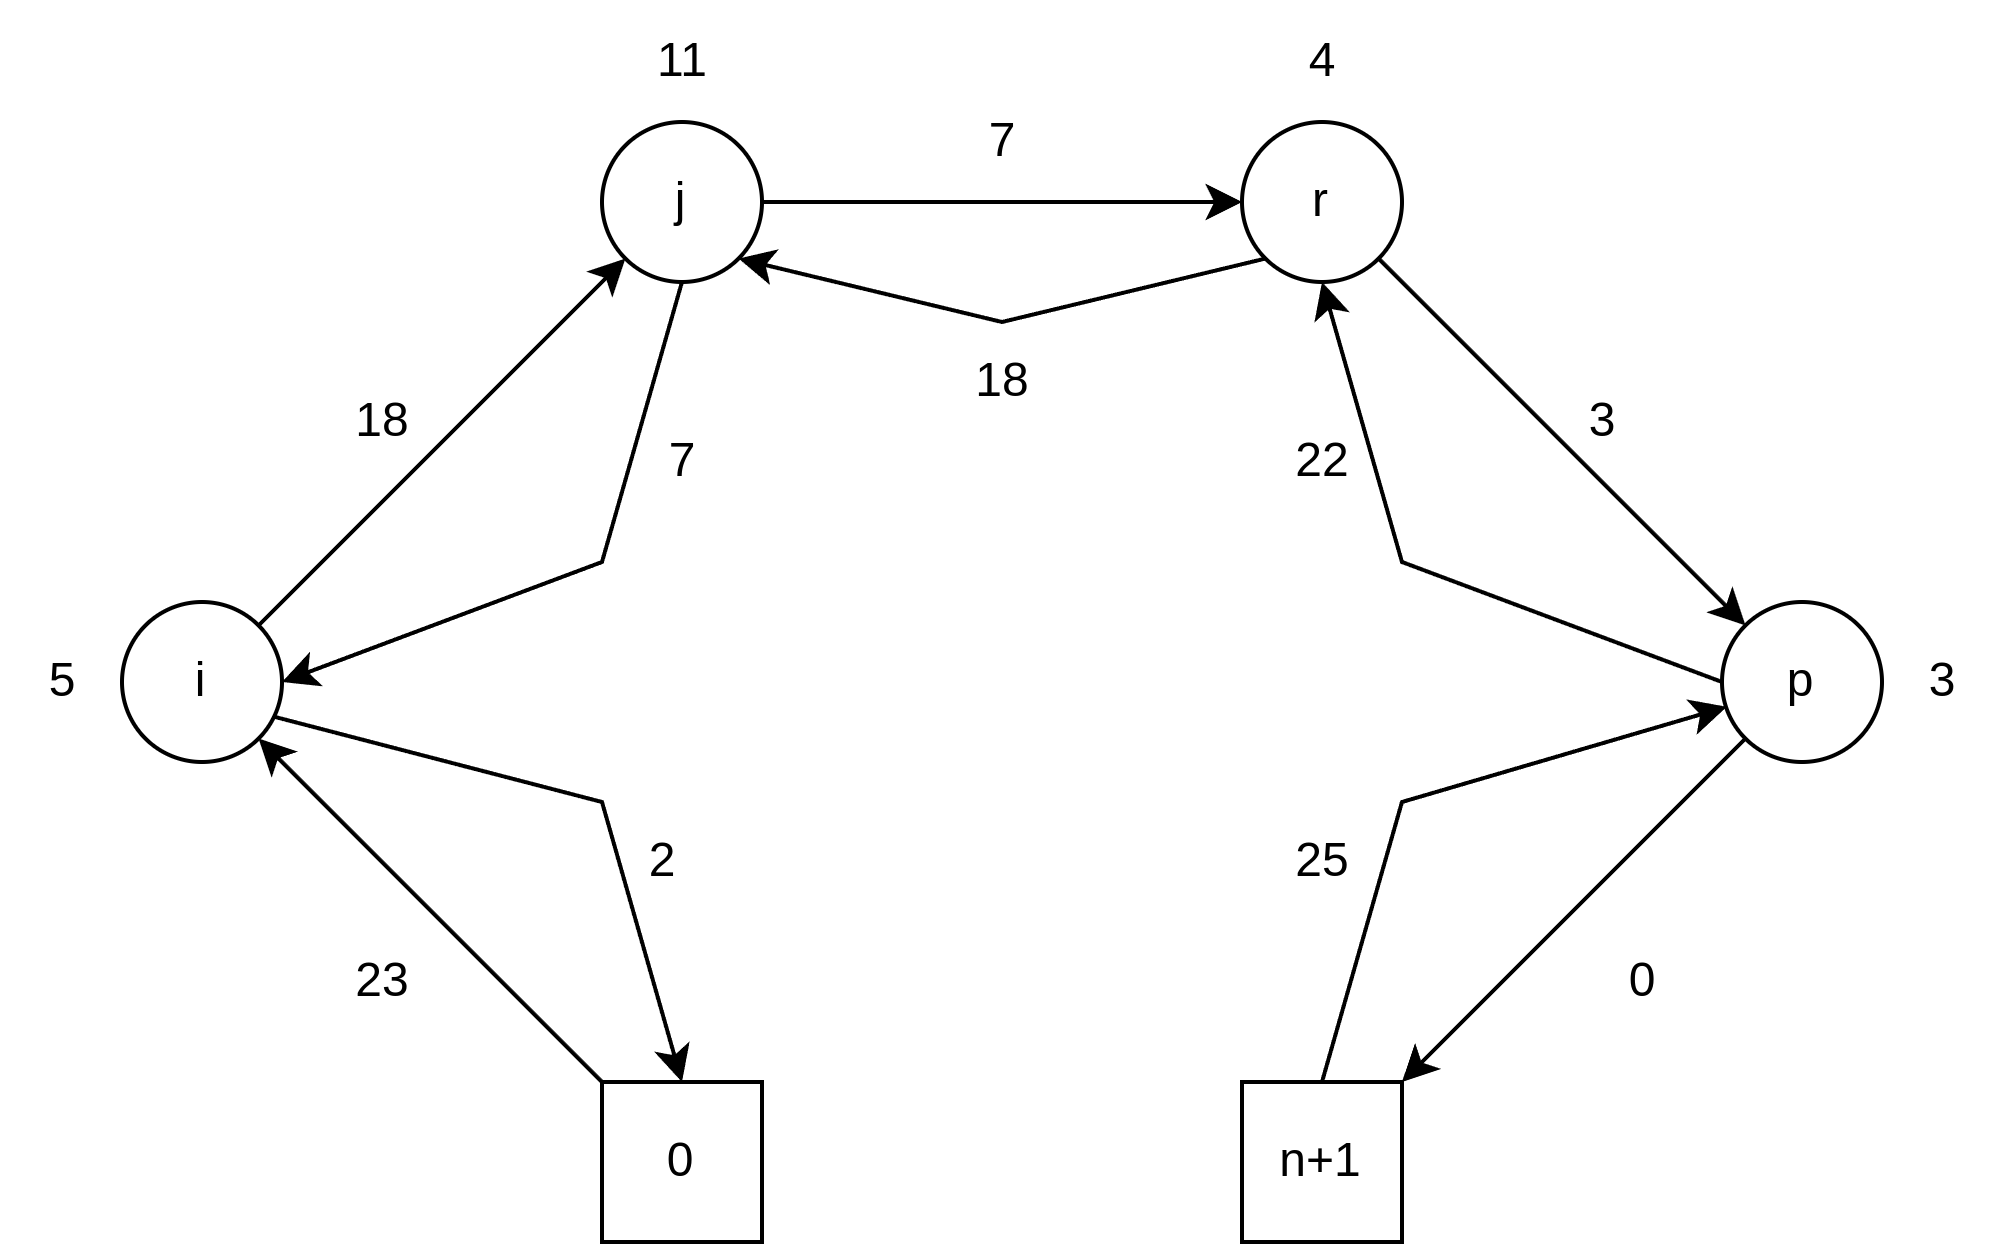
\includegraphics[width=0.8\textwidth]{figures/commondity-flow-model.png} 
  % \includesvg[scale=1]{figures/core-object}
  \caption{Minh họa dòng hàng với $Q=25$} 
  % \label{fig:fg_02}
\end{figure}

\subsection{Công thức phân hoạch tập hợp và thuật toán}
Công thức phân hoạch tập hợp đơn giản của VRP lần đầu được nghiên cứu bởi Balinski, Quandt (1964) \cite{balinski1964integer}. Gọi $r$ là một tuyến, $a_{ir}$ là hệ số nhị phân có giá trị bằng $1$ khi và chỉ khi nút $i \in V \setminus \{0\}$ thuộc tuyến $r$, gọi $c^*$ là chi phí tối ưu của tuyến $r$ và gọi $y_k$ la biến nhị phân bằng $1$ khi và chỉ khi tuyến $r$ được dùng trong lời giải tối ưu. Bài toán được mô hình hóa như sau

\begin{equation}
	\min \sum_r{c_r^* y_r}
\end{equation}
s.t.
\begin{flalign}
	\label{ct4:1} & \sum_r a_{ir} = 1 & \quad (i \in V \setminus \{0\}), \\
	\label{ct4:2} & \sum_r y_r = m,   & \quad                            \\
	\label{ct4:3} & y_r = 0, 1        & \quad (\text{mọi } r).
\end{flalign}

Nói một cách chặt chẽ thì ràng buộc (\ref{ct4:2}) không phải một phần của công thức phân hoạch tập hợp chuẩn, tuy nhiên nó được sử dụng bởi hầu hết các nhà nghiên cứu trong trường hợp VRP.

\section{Heuristics cổ điển}

Nhìn chung thì các thuật toán giải chính xác khó đảm bảo hiệu năng trong thực tế khi mà các tập dữ liệu ngày các lớn và các doanh nghiệp cần phục vụ khách hàng một cách nhanh chóng và tiết kiệm. Thực tế người ta cần tìm ra một (số) lời giải chập nhận được đủ tốt trong một khoảng thời gian "hợp lý". Từ những năm 1964 cho đến 1990, rất nhiều heuristics được nghiên cứu. Một số ít là đưa ra thuật toán hoàn toàn mới còn hầu hết là cải tiến thuật toán đã có.

\subsection{Thuật toán tiết kiệm}

Thuật toán tiết kiệm được đưa ra bởi Clark, Wright (1964) \cite{clarke1964scheduling}, mô tả và cài đặt khá đơn giản nhưng vẫn đưa ra được nghiệm tốt. Chính vì thế, thuật toán này được sử dụng rất rộng rãi. Thuật toán bắt đầu với nghiệm ban đầu với $n$ tuyến $(0, i, 0)$ với $i \in V \setminus \{0\}$. Tại mỗi vòng lặp thuật toán nối tuyến kết thúc với $i$ với một tuyến khác bắt đầu với $j$ cực đại hóa đại lượng \textit{tiết kiệm} $s_{ij}=c_{i0} + c_{0j} - c_{ij}$ và lới giải mới thỏa mãn các ràng buộc. Quá trình kết thúc khi không thể nối các tuyến vào nữa.

Một số cải tiến được đề xuất, ví dụ như nhân $c_{ij}$ với một trọng số dương $\lambda$ (Golden, Magnanti, Nguyen (1977) \cite{golden1977implementing}), tối ưu tuyến đường hợp nhất toàn cục thông qua việc sử dụng thuật toán phù hợp (Altinkemer, Gavish (1991) \cite{altinkemer1991parallel} và Wark, Holt (1994) \cite{wark1994repeated}), tăng tốc tính toán (Paessens (1988) \cite{paessens1988savings})...

\subsection{Phân cụm trước, định tuyến sau}

Heuristic phân cụm trước, định tuyến sau của Fisher, Jaikumar (1981) \cite{fisher1981generalized} trước hết đặt $m$ tâm và phân cụm sao cho tổng khoảng cách từ các nút đến tâm của nó là nhỏ nhất và thỏa mãn về ràng buộc tải trọng. Sau đó trên mỗi cụm, tuyến đường được thiết lập bằng cách giải bài toán TSP. Một vài chiến thuật để khởi tạo cũng như lựa chọn tâm cụm được trình bày trong Baker, Sheasby (1999) \cite{baker1999extensions}

\subsection{Heuristics cải tiến}

\section{Metaheuristics}

Metaheuristics có thể được phân lọai thành tìm kiếm lân cận, tìm kiếm phổ biến và cơ chế học. Hầu hết các thuật toán metaheuristics cho VRP đều dựa trên tìm kiếm lân cận và là các phương pháp cải tiến. Các thuật toán tốt nhất khá mạnh mẽ ngay cả khi nghiệm khởi tạo có chất lượng thấp. Một xu hướng chung là thay vì sử dụng chỉ một thuật toán, người ta thường kết hợp nhiều thuật toán lại với nhau. Các thuật toán như vậy được gọi là thuật toán lai.

Tiếp theo tác giả trình bày ý tưởng chính của một số lớp thuật toán metaheurictics.

\subsection{Tìm kiếm cục bộ}

Về cơ bản, tìm kiếm lân cận cố gắng "khám phá" không gian nghiệm bằng cách "di chuyển" quanh nghiệm hiện tại tới một nghiệm khác trong vùng lần cận của nó. Một số phương pháp có thể kể đến như \textit{tabu search} (Glover (1986) \cite{glover1986future}), \textit{simulated annealing} (Kirkpatrick, Gelatt, and Vecchi
(1983) \cite{kirkpatrick1983optimization}), \textit{deterministic annealing} (Dueck, Scheurer
(1990) \cite{dueck1990threshold}; Dueck (1993) \cite{dueck1993new}), \textit{variable neighbourhood search} (Mladenović, Hansen (1997) \cite{mladenovic1997variable}), \textit{large neighbourhood search}(Shaw (1998) \cite{shaw1998using}) và \textit{adaptive large neighbourhood search} (Ropke, Pisinger (2006) \cite{ropke2006adaptive}). Các thành phần chính của tìm kiếm lân cận là các quy tắc để xác định vùng lân cận của một nghiệm và cơ chế để khám phá vùng lân cận đó.

Trong \textit{tabu search} không gian nghiệm được khám phá bằng cách di chuyển từ nghiệm hiện tại đến nghiệm tốt nhất trong một tập con của lân cận của nghiệm đó. Để tránh việc lặp lại các nghiệm, các nghiệm được gán một thuộc tính gắn với nghiệm hiện tại để không được chọn trong một số lần lặp tiếp theo. Một nghiệm trở thành nghiệm tốt nhất trong số các nghiệm đã biết có thuộc tính gắn với thuộc tính hiện tại. Nguyên lý này được trình bày đầu tiên bởi Cordeau, Gendreau, Laporte (1997) \cite{cordeau1997tabu} và hiện nay được biết đến như là phương pháp tìm kiếm dựa trên thuộc tính (Derigs, Kaiser (2007) \cite{derigs2007applying}).

Trong \textit{simulated annealing} một gnhiệm $x$ được chọn ngẫu nhiên trong lân cận $N(x_t)$ của nghiệm hiện tại $x_t$ tại vòng lặp $t$. Nếu hàm mục tiêu $f$ cực tiểu, ta gán $x_{t+1}:=x$ với $f(x_{t+1}) \leq f(x_t)$. Ngược lại gán $x_{t+1}:=x$ với một xác suất $p_t$ và gán $x_{t+1}:=x_t$ với xác suất $1-p_t$. Trong đó, $p_t$ là một hàm giảm theo $t$ và $f(x) - f(x_t)$.

Trong \textit{deterministic annealing}, nghiệm $x$ cũng được chọn ngẫu nhiên trong lân cận $N(x_t)$. Trong thuật toán \textit{threshold-accepting} (Dueck, Scheurer (1990) \cite{dueck1990threshold}), $x_{t+1}:=x$ khi $f(x) < f(x_t) + \theta_1$, với $\theta_1$ là một trọng số dương; ngược lại gán $x_{t+1}:=x_t$. Trong \textit{record-to-record travel} (Dueck (1993) \cite{dueck1993new}), với nghiệm tốt nhất hiện tại $x^*$, gán $x_{t+1}:=x$ nếu $f(x) \leq \theta_2 f(x^*)$, với $\theta_2$ là một trọng số dương; ngược lại gán $x_{t+1}:=x_t$.; ngược lại gán $x_{t+1}=x_t$.

Trong \textit{Variable neighbourhood search} (Mladenović, Hansen (1997) \cite{}), tác giả xem xét một dánh sách được sắp xếp của các lân cận. Thuật toán bắt đầu với một lân cận và chuyển qua lân cận tiếp theo cho đến khi đạt tới nghiệm tối ưu cục bộ. Việc tìm kiếm được khởi tạo lại khi một nghiệm tốt hơn được tìm thấy hoặc tất cả các lân cận đã dược xét qua. \textit{Very large-scale neighbourhood search - LNS} bỏ đi và tạo lại một (vài) phần của nghiệm hiện tại để tìm kiếm nghiệm tốt hơn. Nguyên lí này giống như cơ chế hủy và tạo lại được trình bày bởi Shaw (1998) \cite{shaw1998using}. \textit{Adaptive large neighbourhood search - ALNS} (Ropke, Pisinger (2006) \cite{ropke2006adaptive}) được biết đến như là một phiên bản mạnh mẽ hơn của \textit{large neighbourhood search}, trong đó các thuật toán hủy hay tạo lại được lựa chọn một cách linh hoạt và thích ứng với trạng thái hiện tại của hệ. LNS và ALNS là cảm hứng chính cho luận văn này. Trong các phần tiếp theo tác giả sẽ trình bày chi tiết về ALNS.

\subsection{Tìm kiếm quần thể}

Tìm kiếm quần thể hoạt động với một quần thể các nghiệm. Thuật toán di truyền (Holland (1975) \cite{holland1975adaptation}) là ví dụ tốt nhất cho mô hình này. Tại mỗi vòng lặp, một vài nghiệm cha dược trích xuất từ quần thể hiện tại và kết hợp để tạo ra các nghiệm con. Nghiệm con sau đó được thay bằng những phần tệ nhất trong quần thể nếu điều này cải thiện nghiệm tốt nhất hiện tại. Về cơ bản, thuật toán áp dụng đa dạng hóa các cơ chế, gọi là đột biến cho thế hệ nghiệm con trước khi xem xét việc đưa chúng vào quần thể.


\subsection{Cơ chế học}

Cơ chế học vay mượn ý tưởng từ trí tuệ nhân tạo với mạng thần kinh (neural networks). Thuật toán học hỏi kinh nghiệm và điều chỉnh các trọng số qua các vòng lặp. Ứng dụng với VRP được trình bày bởi Ghaziri (1991) \cite{ghaziri1991solving}; Schumann, Retzko (1995) \cite{schumann1995self}. Thuật toán tối ưu đàn kiến cũng là một dạng khác của cơ chế học. Nó bắt chước hành vi của đàn kiến trong việc tìm thức ăn và để lại vết trên đường đi. Theo thời gian, vết được để lại nhiều hơn trên đường đi ngắn nhất và qua đó, kiến đi theo con đường này. Ứng dụng đầy đủ được trình bày bởi Reimann, Doerner, Hartl (2004) \cite{reimann2004d}


